\paragraph{}
        Le projet PFA a pour objectif de permettre aux élèves la gestion d'un projet dans sa totalité, depuis la création du cahier des charges en réponse à une demande de clients jusqu'à l'implémentation du projet visé. Il aura ainsi permis de travailler sur le cahier des charges d'un projet, ce qui est un exercice constructif auquel nous n'avions jamais encore eu à faire, mais également de travailler dans une équipe conséquente de 7 personnes quand la plupart des projets réalisés dans le cadre de notre cursus se font par équipe de 3 à 4 personnes.

\paragraph{}      
        Le projet PFA effectué est un projet d'imagerie numérique. Son but est de travailler à l'aide d'un logiciel dans une scène virtuelle en trois dimensions, et d'obtenir grâce à cette dernière des images en deux dimensions permettant de recréer une illusion de trois dimensions. Les algorithmes qui auront notamment été étudiés au cours de ce projet permettent l'obtention d'anaglyphes, d'autostéréogrammes, ou encore de folioscopes.
        L'imagerie numérique n'est pas étudiée au cours des deux premières années d'Informatique à l'Enseirb-Matmeca. Ainsi, ce projet constituait une réelle ouverture d'esprit sur un nouveau domaine de l'informatique.
        
\paragraph{}
        Dans ce rapport, nous présenterons dans un premier temps le domaine de la synthèse d'image, les rendus à implémenter dans notre logiciel et les objectifs donnés dans le cahier des charges. Nous parlerons ensuite de la réalisation technique de notre logiciel, depuis les choix effectés pour la programmation et les algorithmes jusqu'au déroulement du projet et aux difficultés rencontrées. Enfin, nous ferons un bilan de cet expérience de gestion de projet, depuis la phase de cahier des charges jusqu'au rendu.

\begin{figure}[h]
	\centering
	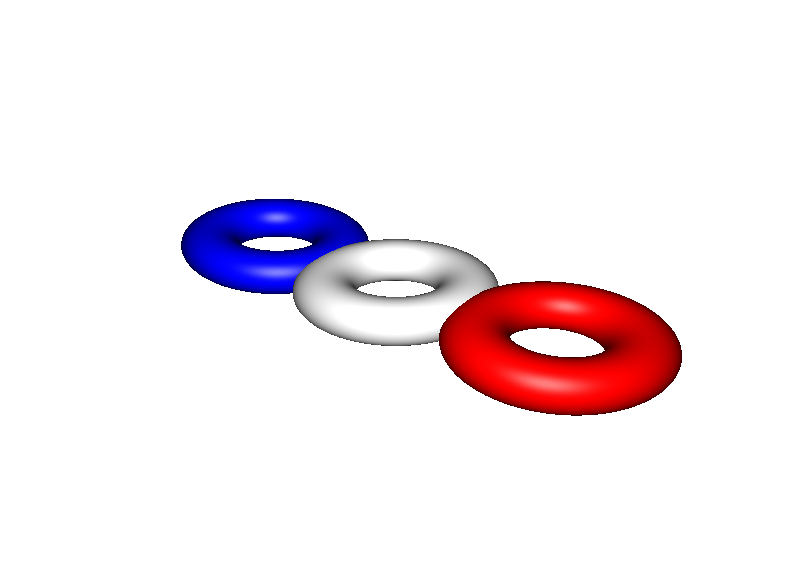
\includegraphics[scale=0.4]{3donut_rendu.png}
	\caption{\label{fig:sphère} Rendu classique du projet \protect}
\end{figure}
